\chapter{Introduction}\label{ch:intro}
\section{Structure of the thesis}
The aim of my thesis is to survey the current state of the art in text generation, especially on the focus of text summarization. For readers who are not familiar with machine learning in general, I will provide a zoom-in introduction into text summarization. My approach is feed-forward from the definition of machine learning, into the natural language processing field, further into the text generation field and within that, I focus on the text summarization part in chapter 1 - Introduction. When research and state of the art results in some natural language processing fields are achieved, those results can often be used across other disciplines as well. For this reason, I provide the most crucial text generation historical achievements in combination with the latest text summarization results, because both topics intersect in many aspects. The crucial concept of historical and modern approaches to summarize and generate text are introduced in chapter 2 - State of the Art. 
To illustrate the basic workflow of a text summarizing system, I programmed a prototype. The concept, development and evaluation of this summarizer are located in chapter 4 - Prototype, but it requires prior knowledge to fully understand the mechanism from the input to the output. Finally in the last chapter I will discuss further improvements for my prototype and a brief discussing into the future of text generation.

\section{Machine Learning}
In the last decade, Machine Learning (ML) is increasingly finding its way into businesses and society. Many websites and businesses use Machine Learning techniques to improve the user and costumer experience. The phrase \textit{Machine Learning} was originally introduced in 1952 by Arthur Samuel. He developed a computer program for playing the game checkers in the 1950s. Samuel's model was based on a model of brain cell interaction by Donald Hebb from his book called \textit{The Organization of Behavior} published in 1949. Hebb's book introduces theories on neuron excitement and the neural communication. Figure \ref{neuron} illustrates the model of the brain cell. Nowadays, this brain neuron based model is mostly declared to be not realistic enough [Andrew Ng, deeplearning.ai], because the structure of a neuron in the brain is far more complex than the illustration in figure \ref{neuron} suggests. Nevertheless, it provides a really good entry point for this research field. 

\begin{figure}
  \begin{center}
  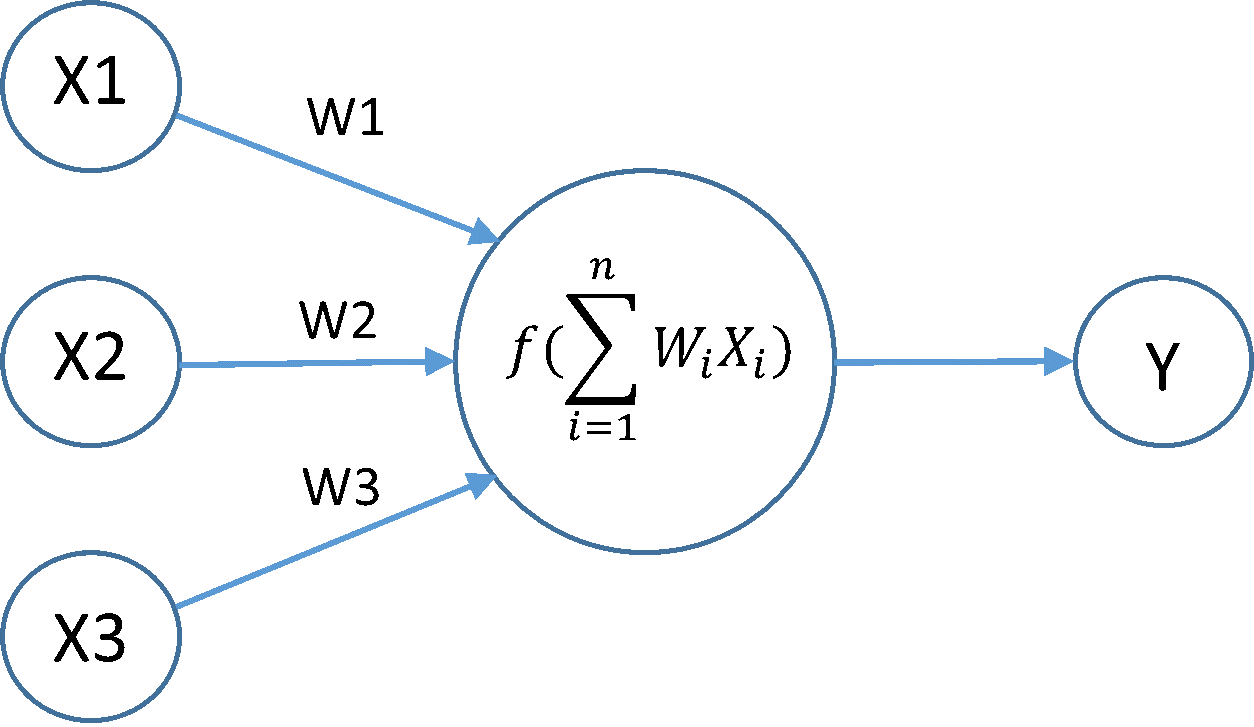
\includegraphics[width=3.5in]{photos/neuron}\\
  \caption{A simple Neuron with 3 inputs and 1 output \cite{neuron}}\label{neuron}
  \end{center}
\end{figure}
 
The roots of Neural Networks (NN) lie down almost 80 years ago in 1943 when \textbf{McCulloch-Pitts} \cite{NN} compared for the first time neuronal networks with the structure of the human brain. The range in which Neural Networks (in the year 2020) apply to modern technologies is wide. Some disciplines have only been created due to the invention of Neural Networks, because they solve existing and new problems very effectively and efficiently. Many frequently held conferences around the globe proof continuous evidence of the successes of Neural Networks. Among those various disciplines counts for example \textit{Pattern recognition} with Convolutional Neural Networks (CNN) \cite{cnn} for example to predict the classes of images with the famous \textit{CIFAR-10} dataset \cite{cifar}. Many amateurs \cite{tim} and experts annually attempt to show their latest results in beating the former best accuracy. 

Convolutional Neural Networks is just one of many other Neural Network building blocks, because a modern network consists of many different layers. Natural Language Processing is one of the various sub fields of Machine Learning. Strictly speaking, it is actually a multidisciplinary field consisting of Artificial Intelligence (AI) and computational linguistics. Natural Language Processing is dedicated to understand and process the interactions between human (natural) language and computers. Natural Language Processing is a very broad term and can apply many different tasks, such as: 

\begin{itemize}
\item Sentiment Analysis
\item Machine Translation
\item Speech Recognition
\item Text Generation (Neural Text Generation \textit{NTG})
\item Chat Bots
\end{itemize}

All of this tasks require many steps to function properly. In the broadest sense, there is always an Input and an Output, which are shown in Table \ref{tab:nlp_table}.

\begin{center} 
	\begin{tabular}{ |p{3cm}||p{3cm}|p{3cm}|p{3cm}|}
		\hline
		\multicolumn{4}{|c|}{\textbf{Components of NLP methods}}\\ \hline\hline
		&Speech &Text &Images \\ \hline
		Input &Speech &Natural Language &Image \\
		Analysis &Recognition  &Processing methods     &Recognition \\ \hline \hline
		Output &Generation &\cellcolor[HTML]{F3E687}Generation &Generation \\
		Synthesis &of Speech & \cellcolor[HTML]{F3E687}of Text &of Images \\ \hline
	\end{tabular}
	\captionof{table}{A closer look into the NLP disciplines}
	\label{tab:nlp_table}
\end{center}

It shows that the text generation is often the output part of a Natural Language Processing model. Data is collected through various different sources, e.g. images, videos or speech, then it is further processed and generates the desired output. Useful examples are shown in Table \ref{tab:nlp_table2}.

\begin{center} 
	\begin{tabular}{ |p{3cm}||p{3cm}|p{3cm}|p{3cm}|}
		\hline
		\multicolumn{4}{|c|}{\textbf{Examples of NLP methods}}\\ \hline\hline
		&Speech &Text &Images \\ \hline
		Input &Siri &Read in &Image \\
		Analysis &listens  &document     &of a face \\ \hline \hline
		Output &Siri &\cellcolor[HTML]{F3E687}Generate &Face \\
		Synthesis &answers & \cellcolor[HTML]{F3E687}Summary &detected \\ \hline
	\end{tabular}
	\captionof{table}{Examples for three different NLP tasks}
	\label{tab:nlp_table2}
\end{center}

For this Bachelor thesis, the focus is on the output part of a Natural Language Processing system, which inputs text as shown in Table \ref{tab:nlp_table} and \ref{tab:nlp_table2}. Text generation is therefore in general the output part of an input-output NLP system.

Another term for text generation is  \textit{Language Modelling}, because text generators use the words of a language and grammar as input for the model. In the past five years, primarly two approaches were used for modelling a Natural Language Processing system, namely the \textbf{rule-based} system and the \textbf{template-based} system (Figure \ref{rules_based}) \cite{NTG2}. Today neural end-to-end systems are \textit{state-of-the-art} \cite{End_to_End}. These systems offer more flexibility and scale with proportionately better results, and less data is required because of the increased complexity. A major disadvantage is that the necessary computing power has increased exponentially. However, this leads to a complex problem because it becomes more and more challenging to understand the decisions of the neural network. The neural network is still, to a large extent, a \textit{black box}. Especially in NLP it gives surprisingly good results. The neural network models for text processing are difficult to understand, so nowadays, compromises between rule-based systems still have to be made, and hybrid systems are most commonly in use. 


\begin{figure}
  \begin{center}
  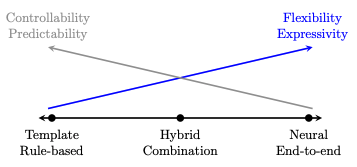
\includegraphics[width=3.5in]{photos/rule_based}\\
  \caption{Rule-Based vs. Neural-Text-Generations System \cite{NTG2}, Page 4}\label{rules_based}
  \end{center}
\end{figure}

When Neural end-to-end systems are used, text generation is often referred as Neural Text Generation (NTG). More examples for Neural Text Generators as output synthetical component are:

\begin{itemize}
\item Speech recording and conversion to text
\item Conversation systems e.g. chatbots
\item Text summary
\item Caption generation
\end{itemize} 


In order to train language models properly, Deep Learning (DL) algorithms teach the model the probabilities of occurring words with respect to the preceding words. There are several approaches to achieve this goal. Language models can be trained on the level of words, whole sentences, or even whole paragraphs. The granularity in which the training takes place is called \textit{n-grams}, where \textit{n} represents the number of preceding words. Further explanation in Section \ref{ss:ngram} of Chapter \ref{ch:sota}. Deep Learning will be explained in necessary depth in Section \ref{ss:history}.



\section{Case study of a Text Summarization System}

Google automated news headline summarization 





